\chapter{Background}
\label{sec:background}

\section{Term Representation and Rewriting}
\label{sec:rewriting}

The most common and easily understood
 program representation is the venerable
 \textit{abstract syntax tree} (AST).
An AST is a recursive tree data structure
 where a node is an operator and
 some number---potentially zero---of children ASTs.
For example, the program $(a * 2) / 2$
 is represented by the AST shown in \autoref{fig:ast1}.
The operators $*$ and $/$ each take two children;
 the variable $a$ and the number $2$ are leaf operators
 that take no children.

ASTs are the primary data structures used in most programming tools,
 but they are not the only ones.
A common alternate representation is the \textit{term graph},
 which can be viewed as a variant of ASTs that
 allows directed acyclic graphs instead of just trees.
Term graphs can therefore capture sharing across common parts of a
 program (also known as a term).
\autoref{fig:ast2} shows a term graph for the program $(a * 2) / 2$.
% Term graphs can be ``unfolded'' into ASTs be duplicating the shared subgraphs,
%  but the resulting ASTs can be exponentially larger than the term graph.

\begin{figure}
  \subcaptionbox{AST without sharing.\label{fig:ast1}}
    [0.5\linewidth]{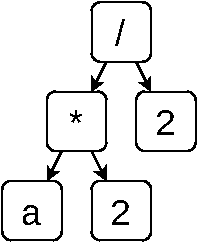
\includegraphics[height=3cm]{ast}}
  \subcaptionbox{Term graph with sharing.\label{fig:ast2}}
    [0.5\linewidth]{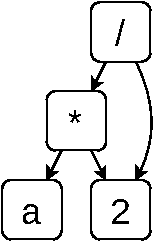
\includegraphics[height=3cm]{ast-sharing}}
  \caption{
    Different representations of the program $(a * 2) / 2$ have
     different characteristics.
    The syntax tree is simpler \subref{fig:ast1},
     but the term graph is smaller since it captures sharing \subref{fig:ast2}.
  }\label{fig:ast}
\end{figure}

Regardless of the choice of program representation,
 a common technique for program manipulation is rewriting.
In this paradigm,
 program transformations are given as a set of rewrites,
 where each
 rewrite $\ell \to r$ specifies a pattern $\ell$ to search for
 and a another pattern $r$ with
 which to replace each instance of $\ell$ found
 in the program.
For example, applying the rewrite $x * 2 \to x + x$
 to our term $(a * 2) / 2$ yields $(a + a) / 2$.

Stated more formally,
 applying rewrite $\ell \to r$ on a term $t$
 works as follows.
First, search for the $\ell$ within $t$,
 yielding a substitution $\sigma$ and a subterm $s$ of $t$
 such that $\sigma$ maps variables from $\ell$ to terms
 and $\ell[\sigma] = s$,
 where $\ell[\sigma]$ denotes replacing the variables in $l$
 with the corresponding terms in $\sigma$.
With the substitution in hand,
 applying the rewrite simply replaces
 $\ell[\sigma]$ with $r[\sigma]$ in $t$
 (since $\ell[\sigma]$ equals some subterm $s$ of $t$).

Rewriting offers an
 intuitive, compositional, and efficient
 method to transform programs
 that is used in programming tools of all shapes and sizes.
It is a well-researched technique with a wealth of literature
 (surveyed in~\cite{nachum-rewrites, rewritesystems}),
 and many programming language tools implement and rely on it.

Term rewriting (in its traditional directed form) does, however,
 suffer from pitfalls that can complicate or prevent the building
 of certain rewrite-based systems.
Many of these weaknesses boil down to the fact that
 term rewriting operates on \emph{one term at a time};
 once a term is rewritten,
 you are left with the new version and have
 essentially forgotten the old version.
The quality of a rewriting system's output can heavily depend on
 the order and manner in which is applies its rewrites.
In other words, \emph{choices really matter} in this paradigm.
The compilers community refers to this as the
 \textit{phase-ordering} problem~\cite{eqsat}.

\begin{figure}
  \centering
  \subcaptionbox{
    Sometimes a locally ``good'' rewrite can be a poor choice down the road.
    In this case, we would ultimately like to rewrite $(a * 2) / 2$ to $2$.
    But applying $x * 2 \to x \ll 1$ is hard to pass up,
     since replacing a (relatively) expensive multiplication with a
     cheap bitshift is nearly always a good decision.
    Applying that locally beneficial rewrite makes canceling out the
     2s much more difficult.\label{fig:bad-rewrites-a}
  }[\linewidth]{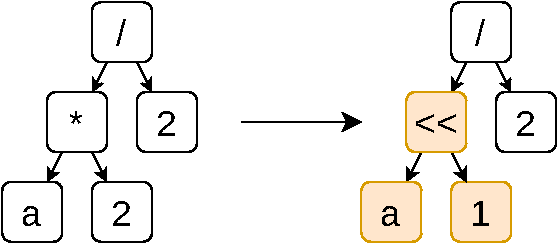
\includegraphics[height=35mm]{figures/bad-rewrites-a}}

  \vspace{1cm}
  \subcaptionbox{
    Seemingly innocuous rewrites like commutativity of multiplication
     ($x * y \to y * x$)
    can send a rewriting system into a loop.
    Directed rewriting systems can avoid this by applying
     these rewrites in only one direction or trying to observe when they have
     encountered a term they have seen before.\label{fig:bad-rewrites-b}
  }[\linewidth]{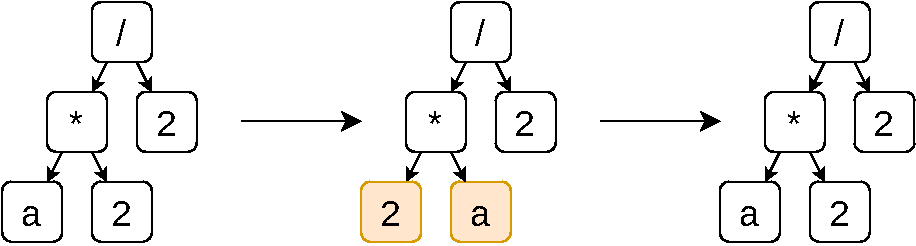
\includegraphics[height=35mm]{figures/bad-rewrites-b}}

  \vspace{1cm}
  \subcaptionbox{
    Expansive rewrites like $x \to x * 1$
     can enable other rewrites,
     but they are problematic for traditional rewriting systems
     since they can always be applied,
     potentially leading to infinitely large terms.
   \label{fig:bad-rewrites-c}
  }[\linewidth]{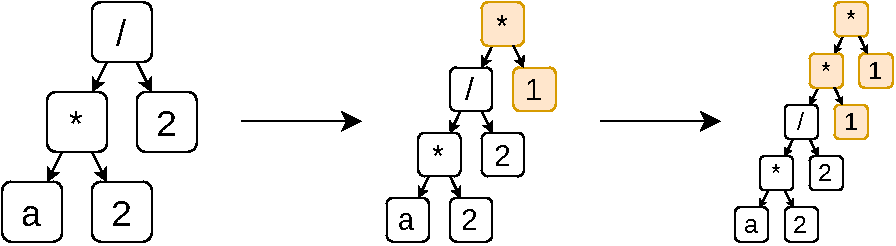
\includegraphics[height=35mm]{figures/bad-rewrites-c}}

  \caption{
    Conventional directed rewriting can go wrong in various ways
    if the wrong rewriting is applied at the wrong time.
    Orange highlighting indicates what changed from the initial term in each subfigure.
  }\label{fig:bad-rewrites}
\end{figure}

\autoref{fig:bad-rewrites} shows some concrete examples of how
 poor rewrite choice can cause undesirable results.


% \section{Term Rewriting}

% \egg builds on \egraphs and equality saturation.
%   This section describes those techniques and
%   presents the challenges that \egg addresses.

% Many problems in program optimization, theorem proving,
%   and other domains have a similar shape:
% given an input expression, search for a ``better'' equivalent
%   expression.
% This paper puts forward the case that, with our proposed advances, equality
%   saturation is now the right tool for the job in many cases like
%   these.

% We will work through an extended example around optimizing
%   the expression
%   $(a \times 2) / 2$
%   and discover the benefits of \egraphs and equality saturation,
%   current limitations of using and implementing this approach,
%   and how \egg addresses those limitations.

\section{E-Graphs}
\label{sec:egraphs}

An \textit{\egraph} is a data structure that stores a set of terms and a
  congruence relation over those terms.
Originally developed for and still used in the
  heart of theorem provers~\cite{nelson, simplify, z3},
  \egraphs have also been used to power a program optimization technique
  called \textit{equality saturation}~%
  \cite{denali, eqsat, eqsat-llvm, szalinski, yogo-pldi20, spores, herbie}.

\subsection{Definitions}

Intuitively,
  an \egraph is a set of equivalence classes (\textit{\eclasses}).
Each \eclass is a set of \textit{\enodes} representing equivalent terms from a given language,
  and an \enode is a function symbol paired with a list of children \eclasses.
More precisely:

\begin{figure}
  \centering
  \begin{align*}
     \text{function symbols} \quad & f,g                                   \\[-0.2em]
     \text{\eclass ids} \quad & a,b & \text{opaque identifiers}            \\[-0.2em]
     \text{terms}     \quad & t  ::= f \mid f(t_1, \ldots, t_m) & m \geq 1 \\[-0.2em]
     \text{\enodes}   \quad & n  ::= f \mid f(a_1, \ldots, a_m) & m \geq 1 \\[-0.2em]
     \text{\eclasses} \quad & c  ::= \{ n_1, \ldots, n_m \}     & m \geq 1
  \end{align*}
  \caption{
    Syntax and metavariables for the components of an \egraph.
    Function symbols may stand alone as constant \enodes and terms.
    An \eclass id is an opaque identifier that can be compared for equality with $=$.
  }
  \label{fig:syntax}
\end{figure}

\begin{definition}[Definition of an E-Graph]
  \label{def:egraph}

  Given the definitions and syntax in \autoref{fig:syntax},
  an \textit{\egraph} is a tuple $(U, M, H)$ where:
  \begin{itemize}
    \item
    A union-find data structure~\cite{unionfind} $U$
      stores an equivalence relation (denoted with $\equivid$)
      over \eclass ids.

    \item
    The \textit{\eclass map} $M$ maps \eclass ids to \eclasses.
    All equivalent \eclass ids map to the same \eclass, i.e.,
      $a \equivid b$ iff $M[a]$ is the same set as $M[b]$.
    An \eclass id $a$ is said to \textit{refer to} the \eclass $M[\find(a)]$.

    \item The \textit{hashcons}\footnote{
      We use the term \textit{hashcons} to evoke the memoization technique,
      since both avoid creating new duplicates of existing objects.
    }
    $H$ is a map from \enodes to \eclass ids.
  \end{itemize}

  % An \textit{\eclass} is a set of \enodes.
  % An \textit{\enode} $f(a_{1}, ..., a_{n})$ is
  %   a function symbol $f$ from the given language
  %   and a (potentially empty) list of \eclass ids.

  Note that an e-class has an identity
   (its canonical \eclass id),
   but an \enode does not.\footnote{
    Our definition of an \egraph reflects \egg's design
      and therefore differs with some other \egraph definitions and implementations.
    In particular, making e-classes but not e-nodes identifiable is unique to
      our definition.
  }
  We use \eclass id $a$ and the \eclass $M[\find(a)]$ synonymously when clear from the context.

\end{definition}

\begin{definition}[Canonicalization]
    An \egraph's union-find $U$ provides a \find operation that canonicalizes \eclass ids
      such that ${\find(U, a) = \find(U, b)}$ iff ${a \equivid b}$.
    We omit the first argument of \find where clear from context.
    \begin{itemize}
      \item An \eclass id $a$ is canonical iff $\find(a) = a$.
      \item \raggedright
            An \enode $n$ is canonical iff $n = \texttt{canonicalize}(n)$,
            where ${\texttt{canonicalize}(f(a_{1}, a_{2}, ...)) = f(\find(a_{1}), \find(a_{2}), ...)}$.
    \end{itemize}
\end{definition}

\begin{definition}[Representation of Terms]
  An \egraph, \eclass, or \enode is said to \textit{represent} a term $t$ if $t$ can be
    ``found'' within it. Representation is defined recursively:
  \begin{itemize}
    \item An \egraph represents a term if any of its \eclasses do.
    \item An \eclass $c$ represents a term if any \enode $n \in c$ does.
    \item An \enode $f(a_{1}, a_{2}, ...)$ represents a term $f(t_{1}, t_{2}, ...)$
          if they have the same function symbol $f$
          and \eclass $M[a_{i}]$ represents term $t_{i}$.
  \end{itemize}

  When each \eclass is a singleton (containing only one \enode),
    an \egraph is essentially a term graph with sharing.
  \autoref{fig:egraph-rewrite1} shows an \egraph that represents the
    expression $(a \times 2) / 2$.
\end{definition}

\begin{definition}[Equivalence]
  An \egraph defines three equivalence relations.
  \begin{itemize}
    \item Over \eclass ids: $a \equivid b$ iff $\find(a) = \find(b)$.
    \item Over \enodes: $n_{1} \equivnode n_{2}$ iff \enodes $n_{1}, n_{2}$ are in the same \eclass,
          i.e., $\exists a.\ n_{1}, n_{2} \in M[a]$.
    \item Over terms: $t_{1} \equivterm t_{2}$ iff terms $t_{1}, t_{2}$ are represented in the same \eclass.
  \end{itemize}

  We use $\equiv$ without the subscript when the relation is clear from context.
\end{definition}

\begin{definition}[Congruence]
  For a given \egraph, let $\cong$ denote a congruence relation over \enodes such that
  ${f(a_{1}, a_{2}, ...) \cong f(b_{1}, b_{2}, ...)}$ iff $a_{i} \equivid b_{i}$.
  Let $\cong^{*}$ denote the congruence closure of $\equivnode$,
   i.e., the smallest superset of $\equivnode$ that is also a superset of $\cong$.
  Note that there may be two \enodes such that
    $n_{1} \cong^{*} n_{2}$ but
    $n_{1} \not\cong n_{2}$ and
    $n_{1} \not\equivnode n_{2}$.
  The relation $\cong$ only represents a single step of congruence;
  more than one step may be required to compute the congruence closure.
\end{definition}

\subsection{E-Graph Invariants}
\label{sec:invariants}

The \egraph must maintain invariants in order to
  correctly and efficiently implement the operations given in \autoref{sec:interface}.
This section only defines the invariants,
  discussion of how they are maintained is deferred to \autoref{sec:rebuild}.
These are collectively referred to as the \textit{e-graph invariants}.

\begin{definition}[The Congruence Invariant]
  \label{def:cong-inv}
  The equivalence relation over \enodes must be closed over congruence,
    i.e., $(\equivnode) = (\cong^{*})$.
  The \egraph must ensure that congruent \enodes are in the same \eclass.
  Since identical \enodes are trivially congruent,
   this implies that an \enode must be uniquely contained in a single \eclass.
\end{definition}

\begin{definition}[The Hashcons Invariant]
  \label{def:hash-inv}
  The hashcons $H$ must map all canonical \enodes to their \eclass ids.
  In other words:
  $$ \enode\ n \in M[a] \iff H[\texttt{canonicalize}(n)] = \find(a) $$
 % for each pair $(n, a) \in H$, \enode $n$ must be canonical and $n \in M[a]$.

  If the hashcons invariant holds, then a procedure $\texttt{lookup}$
    can quickly find which \eclass (if any) has an \enode congruent to a given \enode $n$:
  $\texttt{lookup}(n) = H[\texttt{canonicalize}(n)]$.
\end{definition}

%   \Remy{How can add violate deduplication?}
% Traditionally, \egraphs employ two techniques to maintain the invariants on
%   every call to \texttt{add} or \texttt{merge}.

% As \eclasses grow, the \egraph represents exponentially (or even infinitely) many terms,
%   one for every choice of representative \enode for each \eclass.
% The \egraph in \autoref{fig:egraph-rewrite-before} is essentially an AST with
%   sharing, since each \eclass is a singleton.

% \Egraphs are manipulated by two main operations:
%   adding new \enodes (into new \eclasses)
%   and merging \eclasses (sometimes called \textit{asserting} equivalences).
% \Chandra{since this is POPL, I feel that we might be expected to
% write invariants like the following a bit more formally?}
% These operations maintain two important invariants, which we will call the
%   \textit{\egraph invariants}:
% \begin{enumerate}
%   \item Deduplication:
%     The \egraph must not contain two \enodes with the same operator and
%     equivalent children.
%     \Leo{clarify dedup; distinguish identical and equivalent}
%     \Leo{this doesn't necessarity hold in modern \egraphs}
%   \item Congruence:
%     The equivalence relation on terms must also be a congruence relation, i.e.
%     if $a = b$ then $f(a) = f(b)$.
% \end{enumerate}

% Both operations can violate the two \egraph's congruence invariant.

% Deduplication is typically maintained by \textit{hashconsing}, or memoizing,
%   the add operation.
% If the user tries to add an \enode that is already represented in the \egraph,
%   the \egraph should simply return the \eclass representing the \enode instead of
%   inserting the \enode.
% Congruence is traditionally maintained by keeping a list of
%   \textit{parent pointers} for each \eclass that stores which \enodes have that
%   \eclass as children.
% On the merge operation, the parents of the merged classes must be checked to see
%   if any pairs of them became equivalent, proceeding recursively until no
%   additional equivalences are found.

\begin{figure}
  \begin{subfigure}[t]{0.45\linewidth}
    \centering
    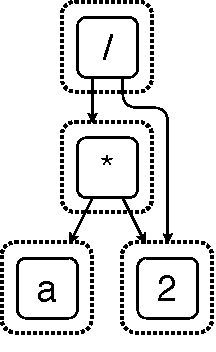
\includegraphics[height=50mm]{overview1.pdf}
    \caption{Initial \egraph contains ${(a \times 2) / 2}$.}
    \label{fig:egraph-rewrite1}
  \end{subfigure}
  \hfill
  \begin{subfigure}[t]{0.45\linewidth}
    \centering
    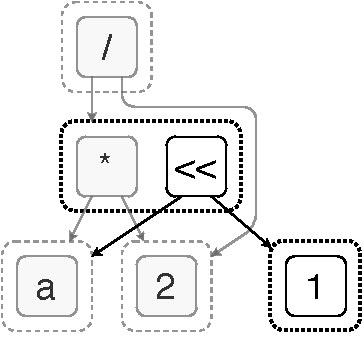
\includegraphics[height=50mm]{overview2.pdf}
    \caption{
      Applied ${x \times 2 \to x \ll 1}$.
    }\label{fig:egraph-rewrite2}
  \end{subfigure}
  \\[1em]
  \begin{subfigure}[t]{0.45\linewidth}
    \centering
    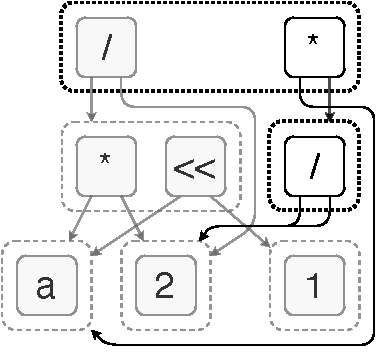
\includegraphics[height=50mm]{overview3.pdf}
    \caption{
      Applied rewrite ${(x \times y) / z \to x \times (y / z)}$.
    }\label{fig:egraph-rewrite3}
  \end{subfigure}
  \hfill
  \begin{subfigure}[t]{0.45\linewidth}
    \centering
    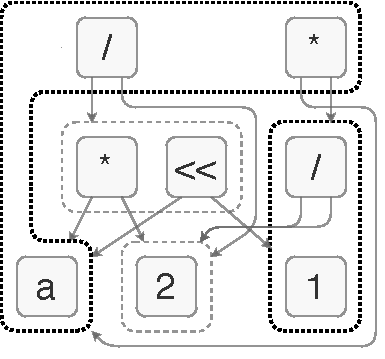
\includegraphics[height=50mm]{overview4.pdf}
    \caption{
      Applied ${x / x \to 1}$ and ${1 \times x \to x}$.
    }\label{fig:egraph-rewrite4}
  \end{subfigure}
  \caption{
    An \egraph consists of \eclasses (dashed boxes) containing
      equivalent \enodes (solid boxes).
    Edges connect \enodes to their child \eclasses.
    Additions and modifications are emphasized in black.
    Applying rewrites to an \egraph adds new \enodes and edges,
      but nothing is removed.
    Expressions added by rewrites are merged with the matched \eclass.
    In \autoref{fig:egraph-rewrite4}, the rewrites do not add any new nodes,
      they only merge \eclasses;
      so the \egraph gets \emph{smaller} but represents \emph{more} terms.
    Since the resulting \egraph has a cycle,
      it actually represents infinitely many expressions:
      $a$, $a \times 1$, $a \times 1 \times 1$, and so on.
  }
  \label{fig:egraph-rewrite}
\end{figure}

\subsection{Interface and Rewriting}
\label{sec:interface}

\Egraphs bear many similarities to the classic union-find data
  structure that they employ internally,
  and they inherit much of the terminology.
\Egraphs provide two main low-level mutating operations:
\begin{itemize}
    \item \texttt{add} takes an \enode $n$ and:
    \begin{itemize}
        \item if $\texttt{lookup}(n) = a$, return $a$;
        \item if $\texttt{lookup}(n) = \emptyset$,
              then set $M[a] = \{ n \}$ and return the id $a$.
    \end{itemize}
    \item \texttt{merge} (sometimes called \texttt{assert} or \texttt{union})
    takes two \eclass ids $a$ and $b$,
    unions them in the union-find $U$,
    and combines the \eclasses by setting both $M[a]$ and $M[b]$ to $M[a] \cup M[b]$.
\end{itemize}

Both of these operations must take additional steps to maintain the congruence
  invariant.
Invariant maintenance is discussed in \autoref{sec:rebuilding}.

\Egraphs also offers operations for querying the data structure.
\begin{itemize}
    \item \texttt{find} canonicalizes \eclass ids using the union-find $U$ as described in definition \ref{def:egraph}.
    \item \texttt{ematch} performs the
          \textit{e-matching}~\cite{simplify, ematching}
          procedure for finding patterns in the \egraph.
          \texttt{ematch} takes a pattern term $p$ with variable placeholders
          and returns a list of tuples $(\sigma, c)$ where $\sigma$ is a substitution of
          variables to \eclass ids such that $p[\sigma]$ is represented in \eclass $c$.
\end{itemize}
These can be composed to perform rewriting over the
  \egraph.
To apply a rewrite $\ell \to r$ to an \egraph,
  \texttt{ematch}
  finds tuples $(\sigma, c)$ where \eclass $c$ represents $\ell[\sigma]$.
Then, for each tuple,
  \mbox{\texttt{merge($c$, add($r[\sigma]$))}} adds $r[\sigma]$ to the \egraph
  and unifies it with the matching \eclass c.

\autoref{fig:egraph-rewrite} shows an \egraph undergoing a series of rewrites.
Note how the process is only additive; the initial term $(a \times 2) / 2$ is
  still represented in the \egraph.
Rewriting in an \egraph can also saturate, meaning the \egraph has
  learned every possible equivalence derivable from the given rewrites.
% This not only solves the phase ordering problem, but also handles rules like
%   commutativity that can be troublesome to a conventional rewrite system.
If the user tried to apply $x \times y \to y \times x$ to an \egraph twice,
  the second time would add no additional \enodes and perform no new merges;
  the \egraph can detect this and stop applying that rule.

\section{Equality Saturation}
\label{sec:eqsat}

Term rewriting~\cite{nachum-rewrites} is a time-tested approach
  for equational reasoning in
  program optimization~\cite{eqsat, denali},
  theorem proving~\cite{simplify, z3},
  and program transformation~\cite{graphs}.
In this setting, a tool repeatedly chooses one of a set of axiomatic rewrites,
  searches for matches of the left-hand pattern in the given
  expression, and replaces matching instances with the substituted
  right-hand side.
It does, however, suffer from drawbacks such as the phase ordering
 problem (\autoref{sec:rewriting}).

% Term rewriting is typically destructive and ``forgets'' the matched
%   left-hand side.
% Consider applying a simple strength reduction rewrite:
%   ${ (a \times 2) / 2 \to (a \ll 1) / 2 }$.
% The new term carries no
%   information about the initial term.
% Applying strength reduction at this point prevents us from canceling out $2/2$.
% In the compilers community, this classically tricky question of when to apply
%   which rewrite is called the \textit{phase ordering} problem.

One solution to the phase ordering problem would simply apply all
  rewrites simultaneously, keeping track of every expression seen.
This eliminates the problem of choosing the correct rule, but
  a naive implementation would require space exponential in the number
  of given rewrites.
\textit{Equality saturation}~\cite{eqsat, eqsat-llvm} is a technique to do this
  rewriting efficiently using an \egraph.

\begin{figure}
  \centering
  \begin{lstlisting}[language=Python, gobble=4, numbers=left, basicstyle=\small\ttfamily, xleftmargin=40mm]
    def equality_saturation(expr, rewrites):
      egraph = initial_egraph(expr)

      while not egraph.is_saturated_or_timeout():

        for rw in rewrites:
          for (subst, eclass) in egraph.ematch(rw.lhs):
            eclass2 = egraph.add(rw.rhs.subst(subst))
            egraph.merge(eclass, eclass2)

      return egraph.extract_best()
  \end{lstlisting}
  \caption{
    Pseudocode for equality saturation.
    Traditionally, equality saturation maintains the \egraph data structure
      invariants throughout the algorithm.
  }
  \label{fig:eq-sat-bg}
\end{figure}

\autoref{fig:eq-sat-bg} shows the equality saturation workflow.
First, an initial \egraph is created from the input term.
The core of the algorithm runs a set of rewrite rules until the \egraph is
  saturated (or a timeout is reached).
Finally, a procedure called \textit{extraction} selects the optimal represented
  term according to some cost function.
For simple cost functions, a bottom-up, greedy traversal of the \egraph suffices
  to find the best term.
Other extraction procedures have been explored for more complex cost
  functions~\cite{spores, wu_siga19}.

Equality saturation eliminates the tedious and often error-prone
  task of choosing when to apply which rewrites,
%Equality saturation turns a correctness problem into a performance problem,
  promising an appealingly simple workflow: state the
  relevant rewrites for the language, create an initial \egraph from a given
  expression, fire the rules until saturation,
  and finally extract the cheapest equivalent expression.
Unfortunately, the technique remains ad hoc; prospective equality saturation
  users must implement their own \egraphs customized to their language, avoid
  performance pitfalls, and hack in the ability to do interpreted reasoning
  that is not supported by purely syntactic rewrites.
\egg aims to address each aspect of these difficulties.

\section{Equality Saturation and Theorem Proving}

An equality saturation engine and a theorem prover each have capabilities that
  would be impractical to replicate in the other.
Automated theorem provers like satisfiability modulo theory (SMT) solvers are
  general tools that, in addition to supporting satisfiability queries,
  incorporate sophisticated, domain-specific solvers to allow interpreted
  reasoning within the supported theories.
On the other hand, equality saturation is specialized for optimization, and its
  extraction procedure directly produces an optimal term with respect to a given
  cost function.
% To replicate extraction with an SMT solver, one would have to resort to a more
%   expensive enumerative approach.

% \James{What enumerative approach? How do you know that one would "have to" resort to it?}

While SMT solvers are indeed the more general tool,
  equality saturation is not superseded by SMT;
  the specialized approach can be much faster when the full generality of SMT is
  not needed.
To demonstrate this, we replicated a portion of the recent TASO paper~\cite{taso},
  which optimizes deep learning models.
As part of the work, they must verify a set of synthesized equalities with
  respect to a trusted set of universally quantified axioms.
TASO uses Z3~\cite{z3} to perform the
  verification even though most of Z3's features
  (disjunctions, backtracking, theories, etc.)
  were not required.
An equality saturation engine can also be used for verifying these equalities
  by adding the left and right sides of
  each equality to an \egraph,
  running the axioms as rewrites,
  and then checking if both sides end up in the same \eclass.
Z3 takes 24.65 seconds to perform the verification;
  \egg performs the same task in 1.56 seconds ($15\times$ faster),
  or only 0.52 seconds ($47\times$ faster) when using
  \egg's batched evaluation (\autoref{sec:egg-batched}).

% \James{
  % The experimental/perf numbers in the last par of 2.4 feel out of place. Not sure how to fix...
% }

% However, their abilities overlap on a specific kind of theorem proving:
%   given a list of axioms in the form of universal quantified equalities,
%   prove two (or more) terms equal.
% Some SMT solvers support these kinds of queries, albeit in a limited fashion
%   since they are undecidable.
% \footnotetext{
%   Since these queries are undecidable, both SMT solvers and equality
%   saturation engines can either prove the inputs equal or fail to; they cannot
%   prove them unequal.
% }



%%% Local Variables:
%%% TeX-master: "../thesis"
%%% End:
